\chapter{Resultados}
\label{chap:resultados}

Este capítulo apresenta os resultados obtidos a partir da aplicação da metodologia descrita anteriormente. A análise está estruturada de forma a construir uma compreensão progressiva dos fatores que influenciam o desempenho dos atletas na prova, partindo de uma análise descritiva geral, passando pela investigação de fatores demográficos e de estratégia, pela identificação de perfis de corredores e, finalmente, culminando na construção de um modelo preditivo.

\section{Análise Descritiva da Amostra}

Após os procedimentos de limpeza, tratamento e agregação dos dados, a amostra final consolidada para análise foi composta por 109 atletas únicos. A variável resposta principal do estudo, o tempo final de prova (\texttt{Tempo\_Final\_min}), apresentou uma considerável variabilidade, como detalhado na Tabela \ref{tab:descritiva_geral} e ilustrado na Figura \ref{fig:dist_tempo_final}.

% --- Tabela Descritiva Geral ---
\begin{table}[]
\centering
\caption{Estatísticas descritivas das principais variáveis de desempenho (N=109).}
\label{tab:descritiva_geral}
\resizebox{\columnwidth}{!}{%
\begin{tabular}{@{}lccc@{}}
\toprule
\textbf{Estatística} & \textbf{Tempo Final (min)} & \textbf{Ritmo Médio (min/km)} & \multicolumn{1}{l}{\textbf{Variabilidade do Ritmo (min)}} \\ \midrule
Média                & 422.00                     & 11.87                         & 7.02                                                      \\
Desvio Padrão        & 122.97                     & 3.50                          & 3.26                                                      \\
Mínimo               & 236.40                     & 6.57                          & 2.90                                                      \\
Mediana              & 389.82                     & 10.82                         & 5.65                                                      \\
Máximo               & 790.93                     & 22.60                         & 16.51                                                     \\ \bottomrule
\end{tabular}%
}
\end{table}
\begin{flushleft}
    \footnotesize Fonte: Elaborado pelo autor (2025).
\end{flushleft}

O tempo médio para completar a prova foi de 422 minutos (aproximadamente 7 horas), com uma grande dispersão nos resultados (desvio padrão de 123 minutos). O atleta mais rápido completou o percurso em 236 minutos (menos de 4 horas), enquanto o último concluinte levou 791 minutos (mais de 13 horas). A Figura \ref{fig:dist_tempo_final} mostra a distribuição dos tempos, que apresenta uma leve assimetria à direita.

% --- Figura Distribuição do Tempo Final ---
\begin{figure}[H]
    \centering
    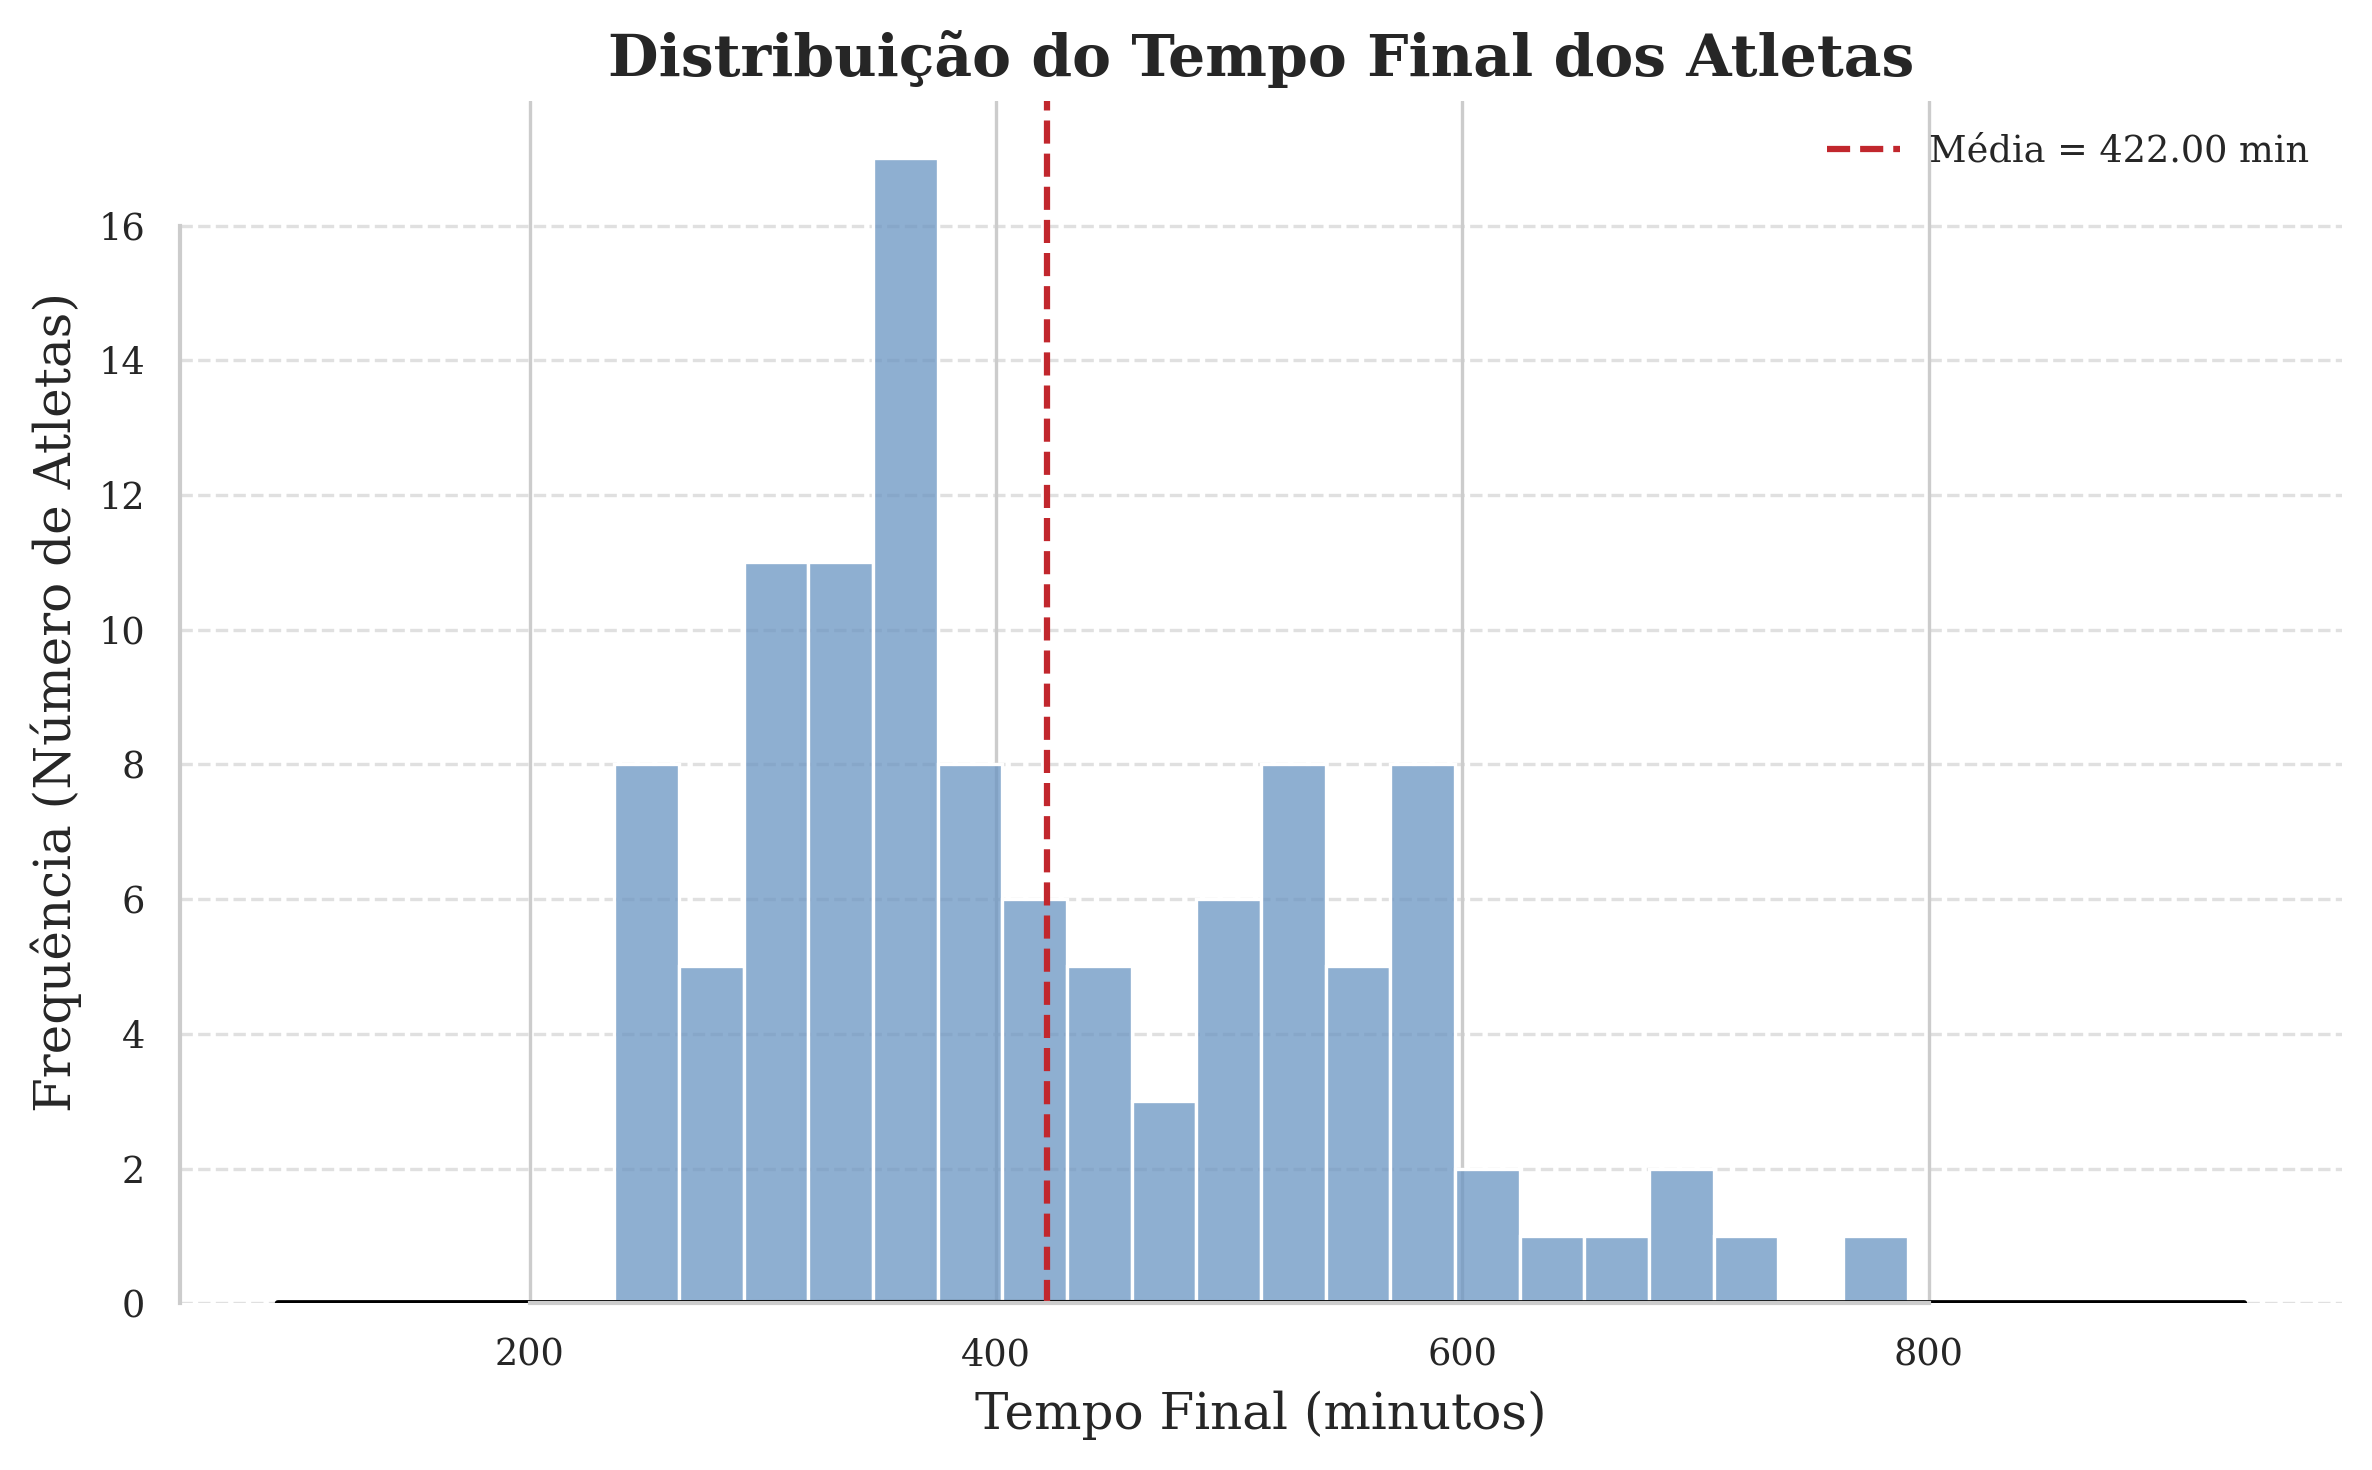
\includegraphics[width=0.8\textwidth]{Imagens/distribuicao_tempo_final.png}
    \caption{Histograma da distribuição do Tempo Final em minutos.}
    \label{fig:dist_tempo_final}
    \caption*{Fonte: Elaborado pelo autor (2025).}
\end{figure}

\section{Análise de Fatores Demográficos}

Nesta seção, investiga-se a relação entre o desempenho e as características demográficas dos atletas: sexo, faixa etária e peso.

\subsection{Influência do Sexo no Desempenho}

A amostra foi composta por 78 homens e 31 mulheres. A análise comparativa revelou uma diferença estatisticamente significativa entre os grupos. O teste de Shapiro-Wilk indicou que a variável \texttt{Tempo\_Final\_min} não seguia uma distribuição normal para ambos os grupos (p=0.0008 para homens e p=0.0360 para mulheres), justificando o uso de um teste não-paramétrico.

O Teste de Mann-Whitney U resultou em um p-valor de \textbf{0.0319}, que, sendo inferior ao nível de significância $\alpha=0.05$, nos leva a rejeitar a hipótese nula. Conclui-se que existe uma diferença estatisticamente significativa no tempo de prova entre homens e mulheres. Conforme observado na Figura \ref{fig:boxplot_sexo} e na Tabela \ref{tab:descritiva_sexo}, os homens apresentaram, em média, um tempo de conclusão menor (média de 405.4 min) em comparação com as mulheres (média de 463.7 min).

% --- Figura Boxplot por Sexo ---
\begin{figure}[H]
    \centering
    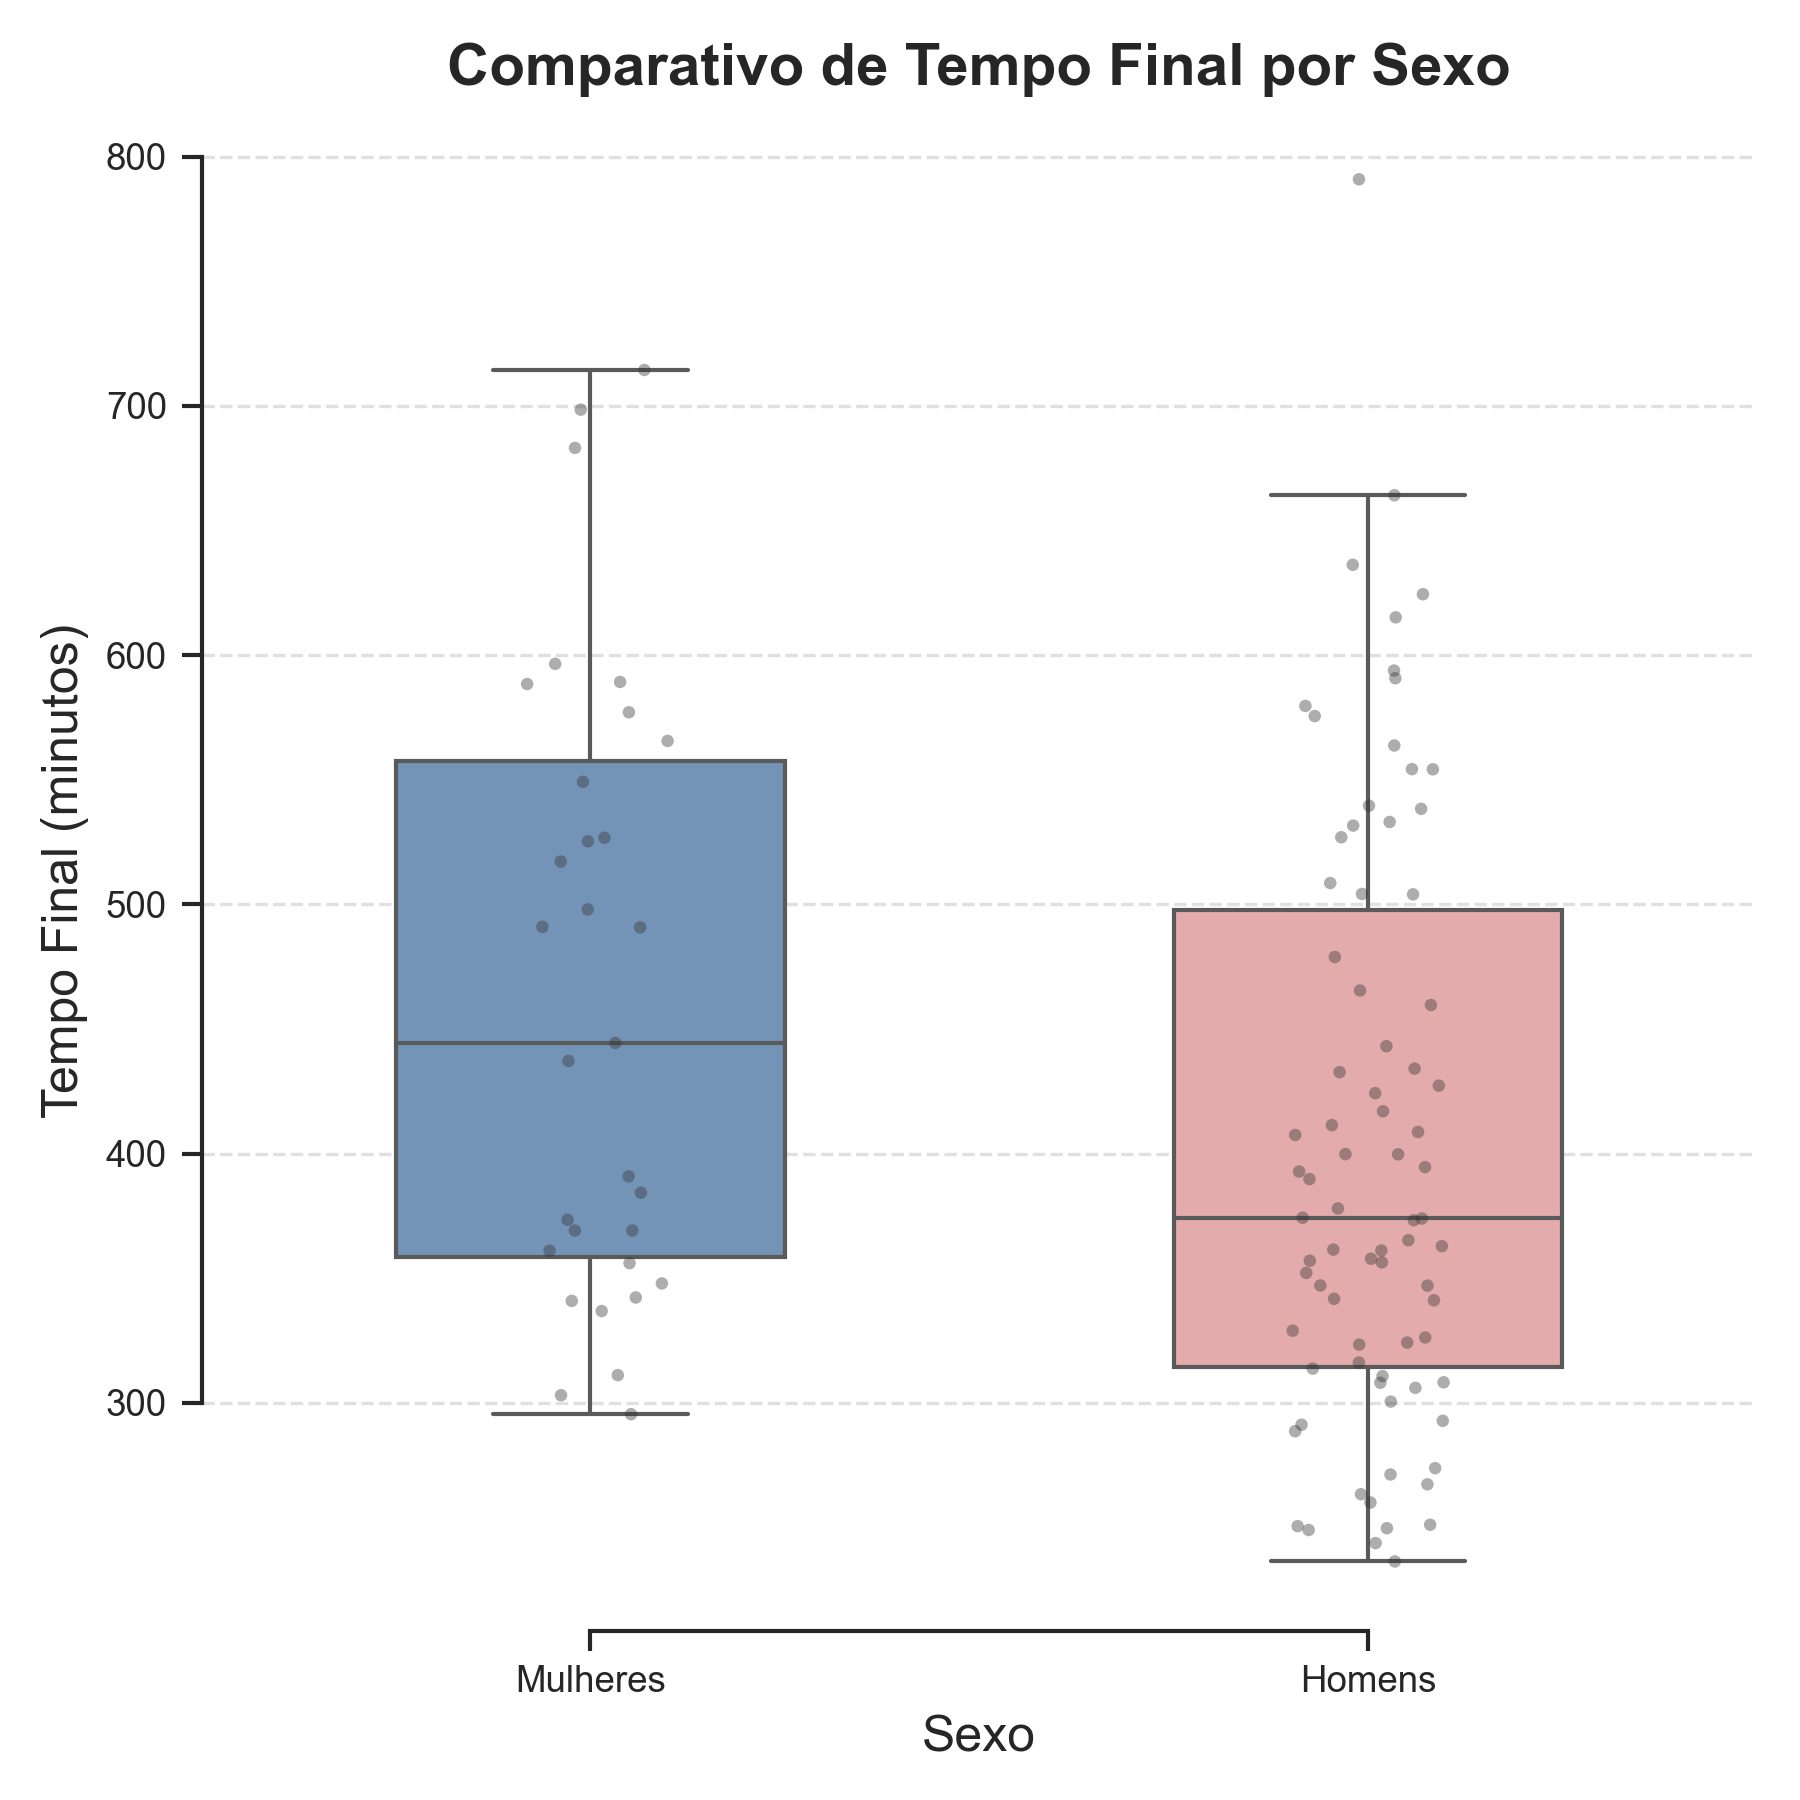
\includegraphics[width=0.8\textwidth]{Imagens/boxplot_tempo_por_sexo.png}
    \caption{Boxplot comparativo do Tempo Final por Sexo.}
    \label{fig:boxplot_sexo}
    \caption*{Fonte: Elaborado pelo autor (2025).}
\end{figure}

% --- Tabela Descritiva por Sexo ---
\begin{table}[H]
\centering
\caption{Estatísticas descritivas do Tempo Final (min) por Sexo.}
\label{tab:descritiva_sexo}
\begin{tabular}{lcc}
\toprule
\textbf{Estatística} & \textbf{Homens} & \textbf{Mulheres} \\
\midrule
Média   & 405.43 & 463.71 \\
Mediana & 374.14 & 444.42 \\
Desvio Padrão & 119.60 & 123.35 \\
N       & 78     & 31     \\
\bottomrule
\end{tabular}
\caption*{Fonte: Elaborado pelo autor (2025).}
\end{table}

\subsection{Influência da Faixa Etária no Desempenho}

Os atletas foram distribuídos em cinco faixas etárias, com maior concentração entre 25 e 44 anos (72\% da amostra). O teste de Shapiro-Wilk apontou que múltiplos grupos não seguiam a normalidade, indicando o Teste de Kruskal-Wallis como a ferramenta adequada. Devido à presença de grupos com amostras pequenas (n=4 e n=6), um Teste de Permutação foi realizado para garantir a robustez do p-valor, resultando em \textbf{p=0.0360}.

Este resultado significativo indica que existe diferença no tempo de prova entre pelo menos duas faixas etárias. Para identificar quais grupos diferem entre si, foi aplicado o teste \textit{post-hoc} de Dunn com correção de Bonferroni (Tabela \ref{tab:dunn_faixa_etaria}).

% --- Figura Boxplot por Faixa Etária ---
\begin{figure}[H]
    \centering
    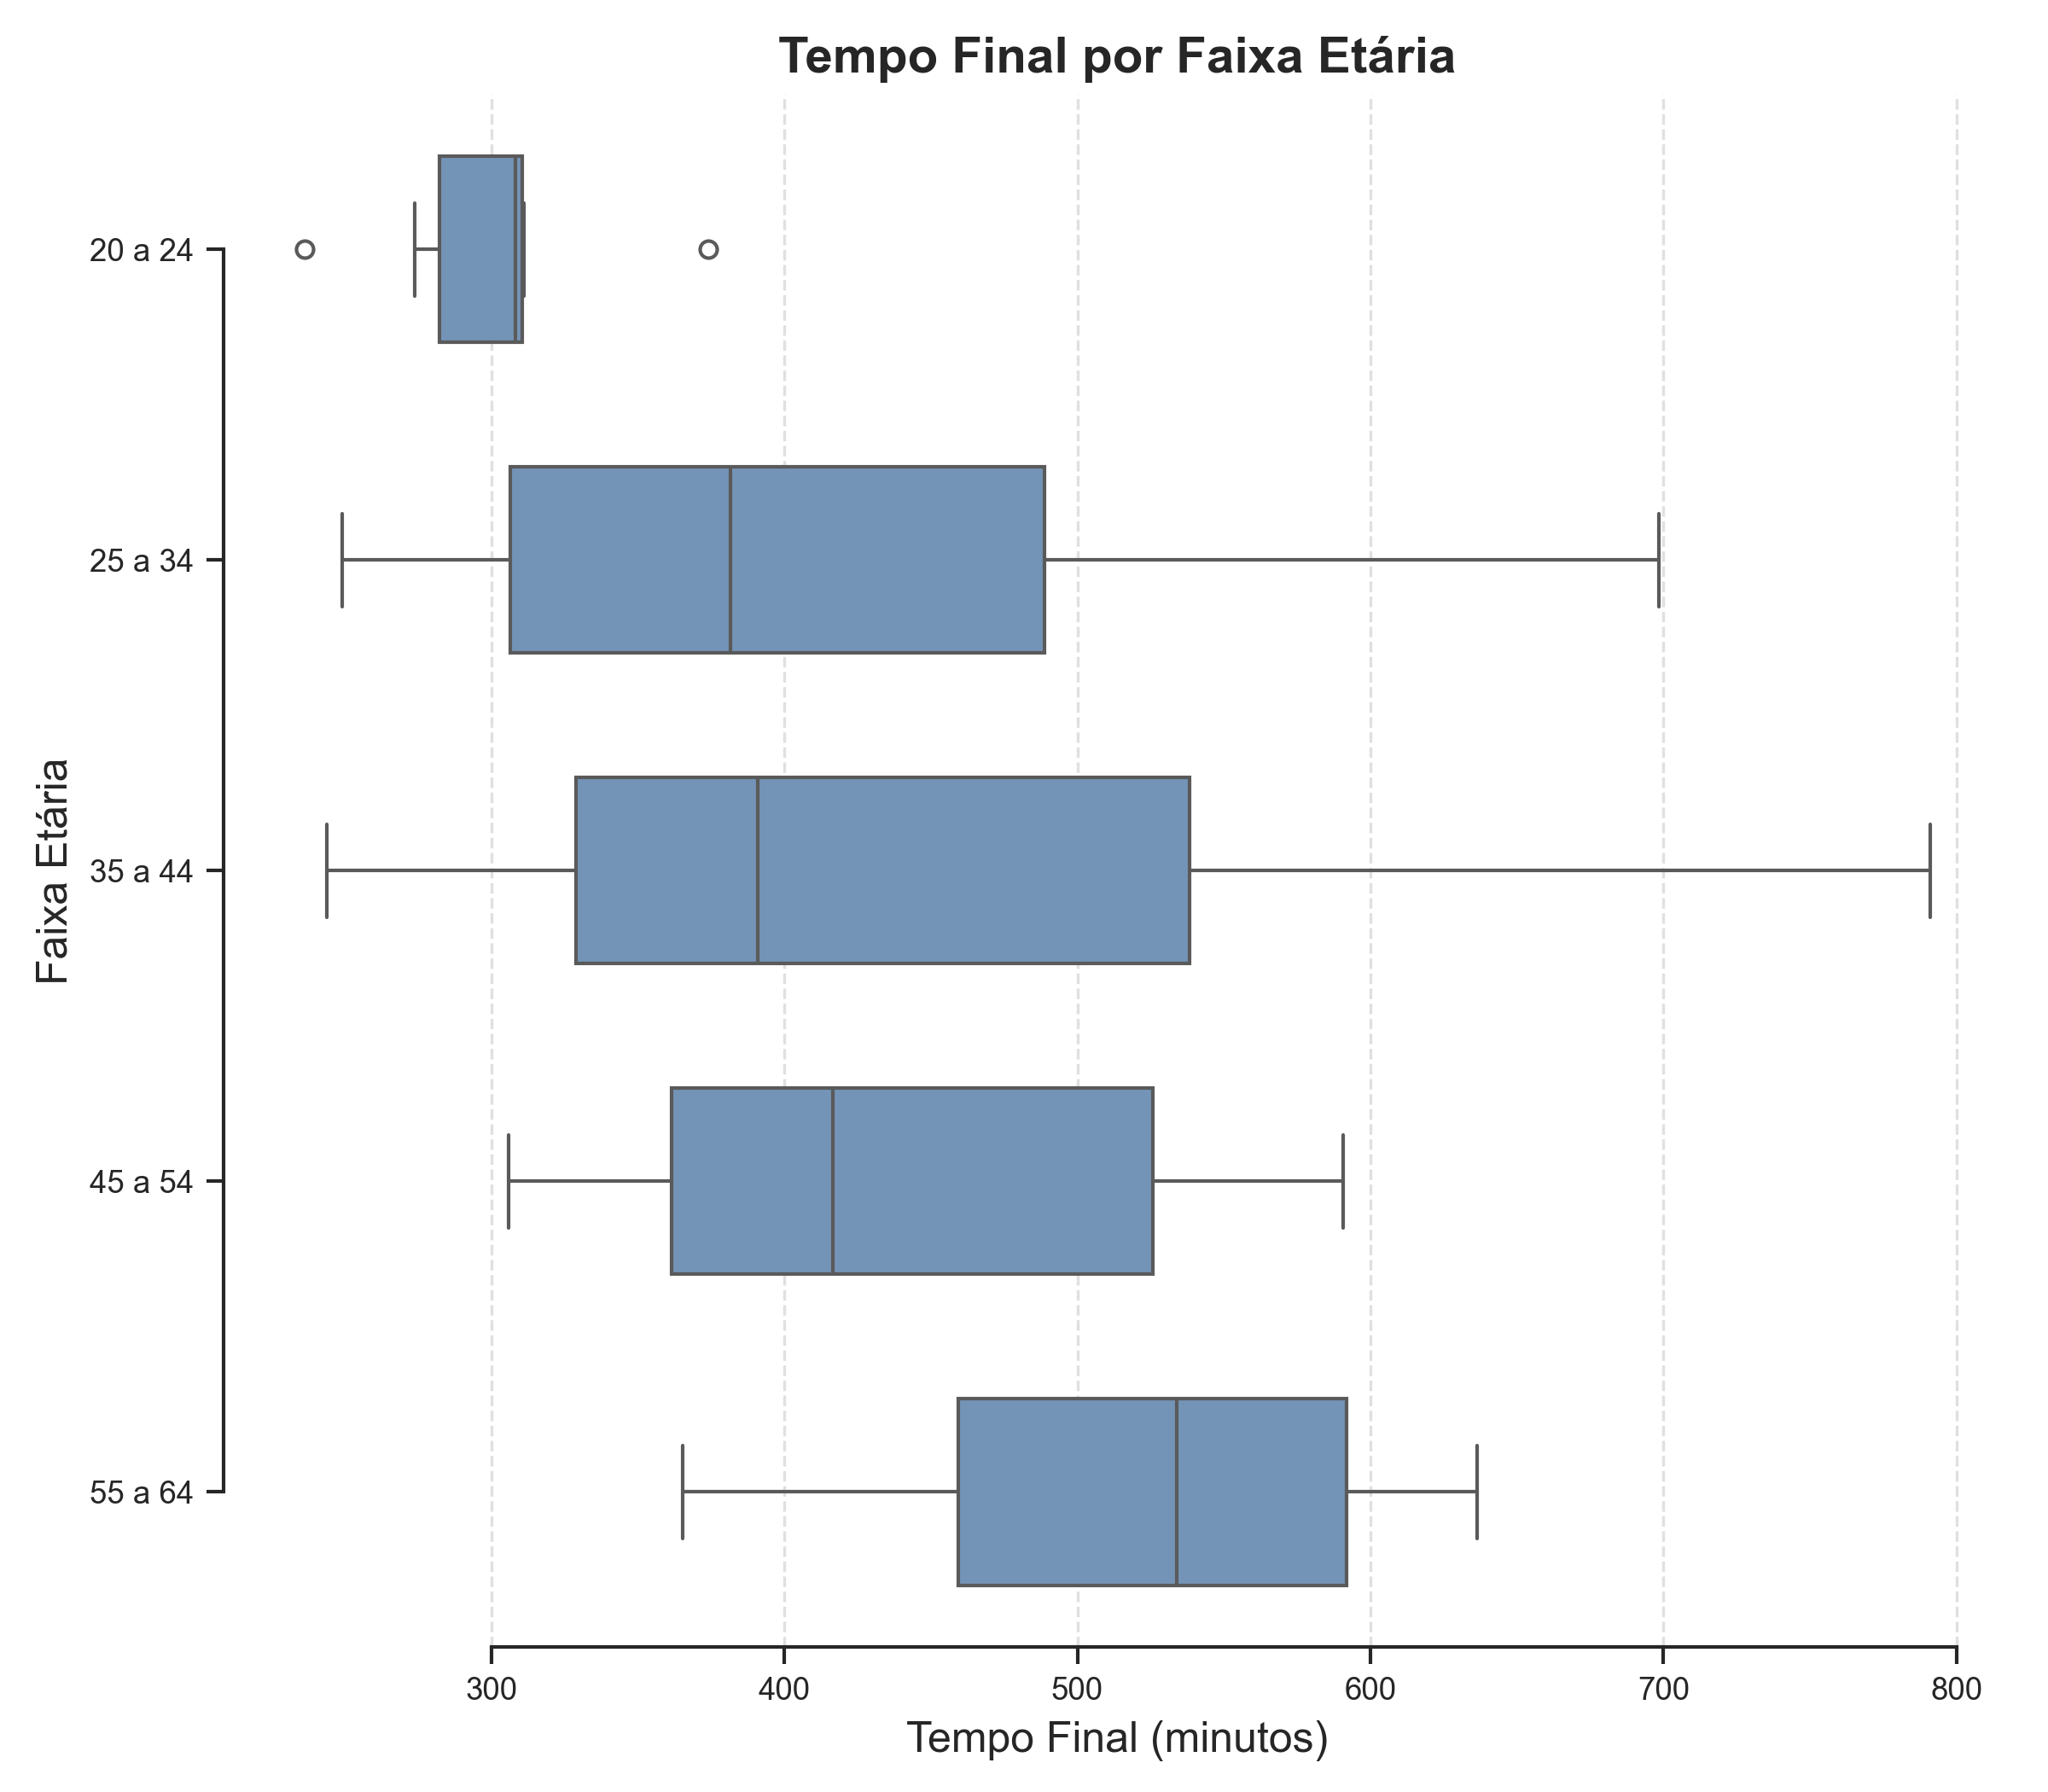
\includegraphics[width=0.8\textwidth]{Imagens/boxplot_tempo_por_faixa_etaria.png}
    \caption{Boxplot comparativo do Tempo Final por Faixa Etária.}
    \label{fig:boxplot_idade}
    \caption*{Fonte: Elaborado pelo autor (2025).}
\end{figure}

% --- Tabela Post-Hoc Dunn ---
\begin{table}[H]
\centering
\caption{Matriz de p-valores do teste \textit{post-hoc} de Dunn com correção de Bonferroni.}
\label{tab:dunn_faixa_etaria}
\begin{tabular}{lccccc}
\toprule
 & \textbf{20 a 24} & \textbf{25 a 34} & \textbf{35 a 44} & \textbf{45 a 54} & \textbf{55 a 64} \\
\midrule
\textbf{20 a 24} & 1.000 & - & - & - & - \\
\textbf{25 a 34} & 0.313 & 1.000 & - & - & - \\
\textbf{35 a 44} & 0.080 & 1.000 & 1.000 & - & - \\
\textbf{45 a 54} & \textbf{0.042} & 1.000 & 1.000 & 1.000 & - \\
\textbf{55 a 64} & \textbf{0.036} & 0.804 & 1.000 & 1.000 & 1.000 \\
\bottomrule
\end{tabular}
\caption*{Fonte: Elaborado pelo autor (2025).}
\end{table}

A análise \textit{post-hoc} revelou que os atletas da faixa \textbf{20 a 24 anos} foram significativamente mais rápidos que os da faixa \textbf{45 a 54 anos (p=0.042)} e os da faixa \textbf{55 a 64 anos (p=0.036)}. Nenhuma outra comparação entre pares de grupos se mostrou estatisticamente significativa.

\subsection{Influência da Faixa de Peso no Desempenho}

Para a análise de peso, categorias com poucos atletas foram agrupadas para garantir a robustez do teste. A categoria "Não informado" foi removida da análise de hipótese. O teste de Shapiro-Wilk novamente indicou a não normalidade em vários grupos, levando à escolha do Teste de Kruskal-Wallis. O resultado do teste foi um \textbf{p-valor de 0.1810}.

Como o p-valor é maior que $\alpha=0.05$, não rejeitamos a hipótese nula. Conclui-se que, para esta amostra, \textbf{não há evidências estatísticas suficientes para afirmar que existe uma diferença no tempo de conclusão da prova entre as diferentes faixas de peso}.

% --- Figura Boxplot por Faixa Etária ---
\begin{figure}[H]
    \centering
    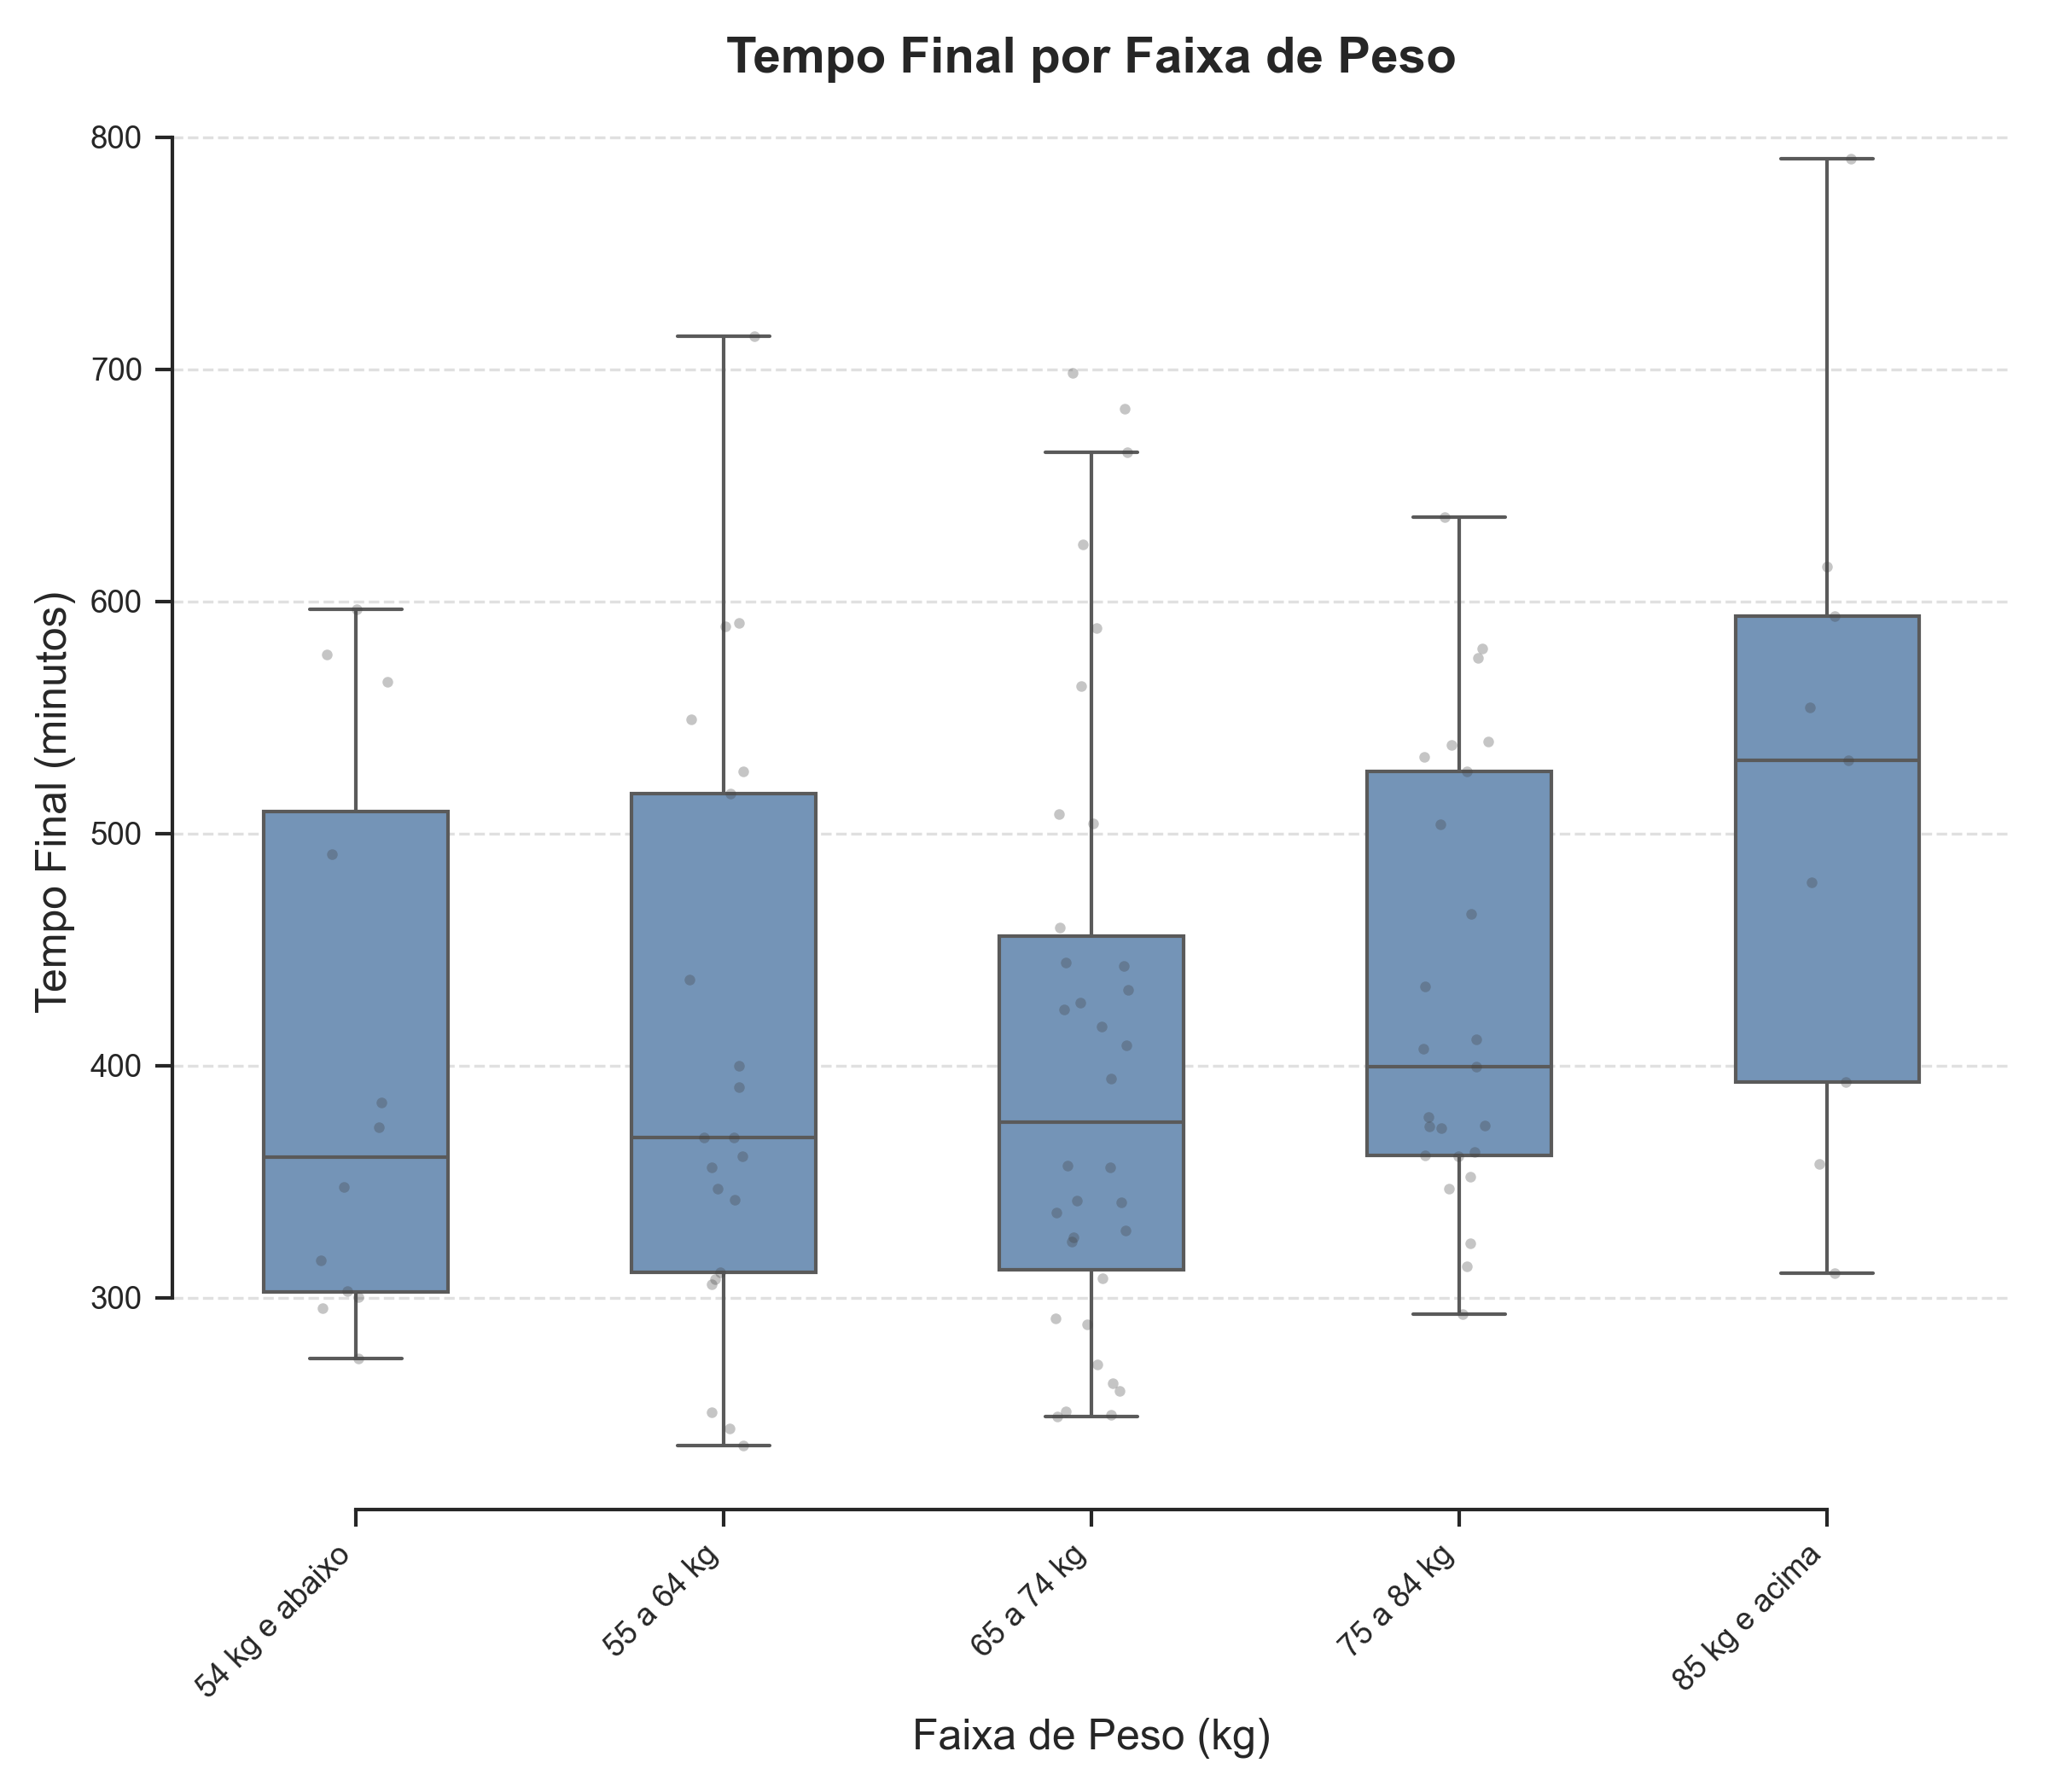
\includegraphics[width=0.8\textwidth]{Imagens/boxplot_tempo_por_peso.png}
    \caption{Boxplot comparativo do Tempo Final por Faixa de Peso.}
    \label{fig:boxplot_peso}
    \caption*{Fonte: Elaborado pelo autor (2025).}
\end{figure}

\section{Análise da Consistência de Ritmo}

A análise da relação entre a consistência do ritmo (\texttt{Variabilidade\_Ritmo\_min\_std}) e o desempenho (\texttt{Tempo\_Final\_min}) foi um ponto central do estudo. Como ambas as variáveis não apresentaram distribuição normal (Shapiro-Wilk com p<0.001 para ambas), optou-se pela \textbf{Correlação de Spearman}.

O resultado revelou um coeficiente \textbf{rho ($\rho$) de 0.9388} com um \textbf{p-valor virtualmente zero ($p \approx 2.44 \times 10^{-51}$)}. Isso indica uma \textbf{correlação positiva muito forte e significativa}. A Figura \ref{fig:scatter_variabilidade} ilustra essa relação de forma clara.

% --- Figura Scatter Plot Variabilidade ---
% COMENTÁRIO: João, insira aqui o arquivo de imagem do seu scatter plot (In [40]).
\begin{figure}[H]
    \centering
    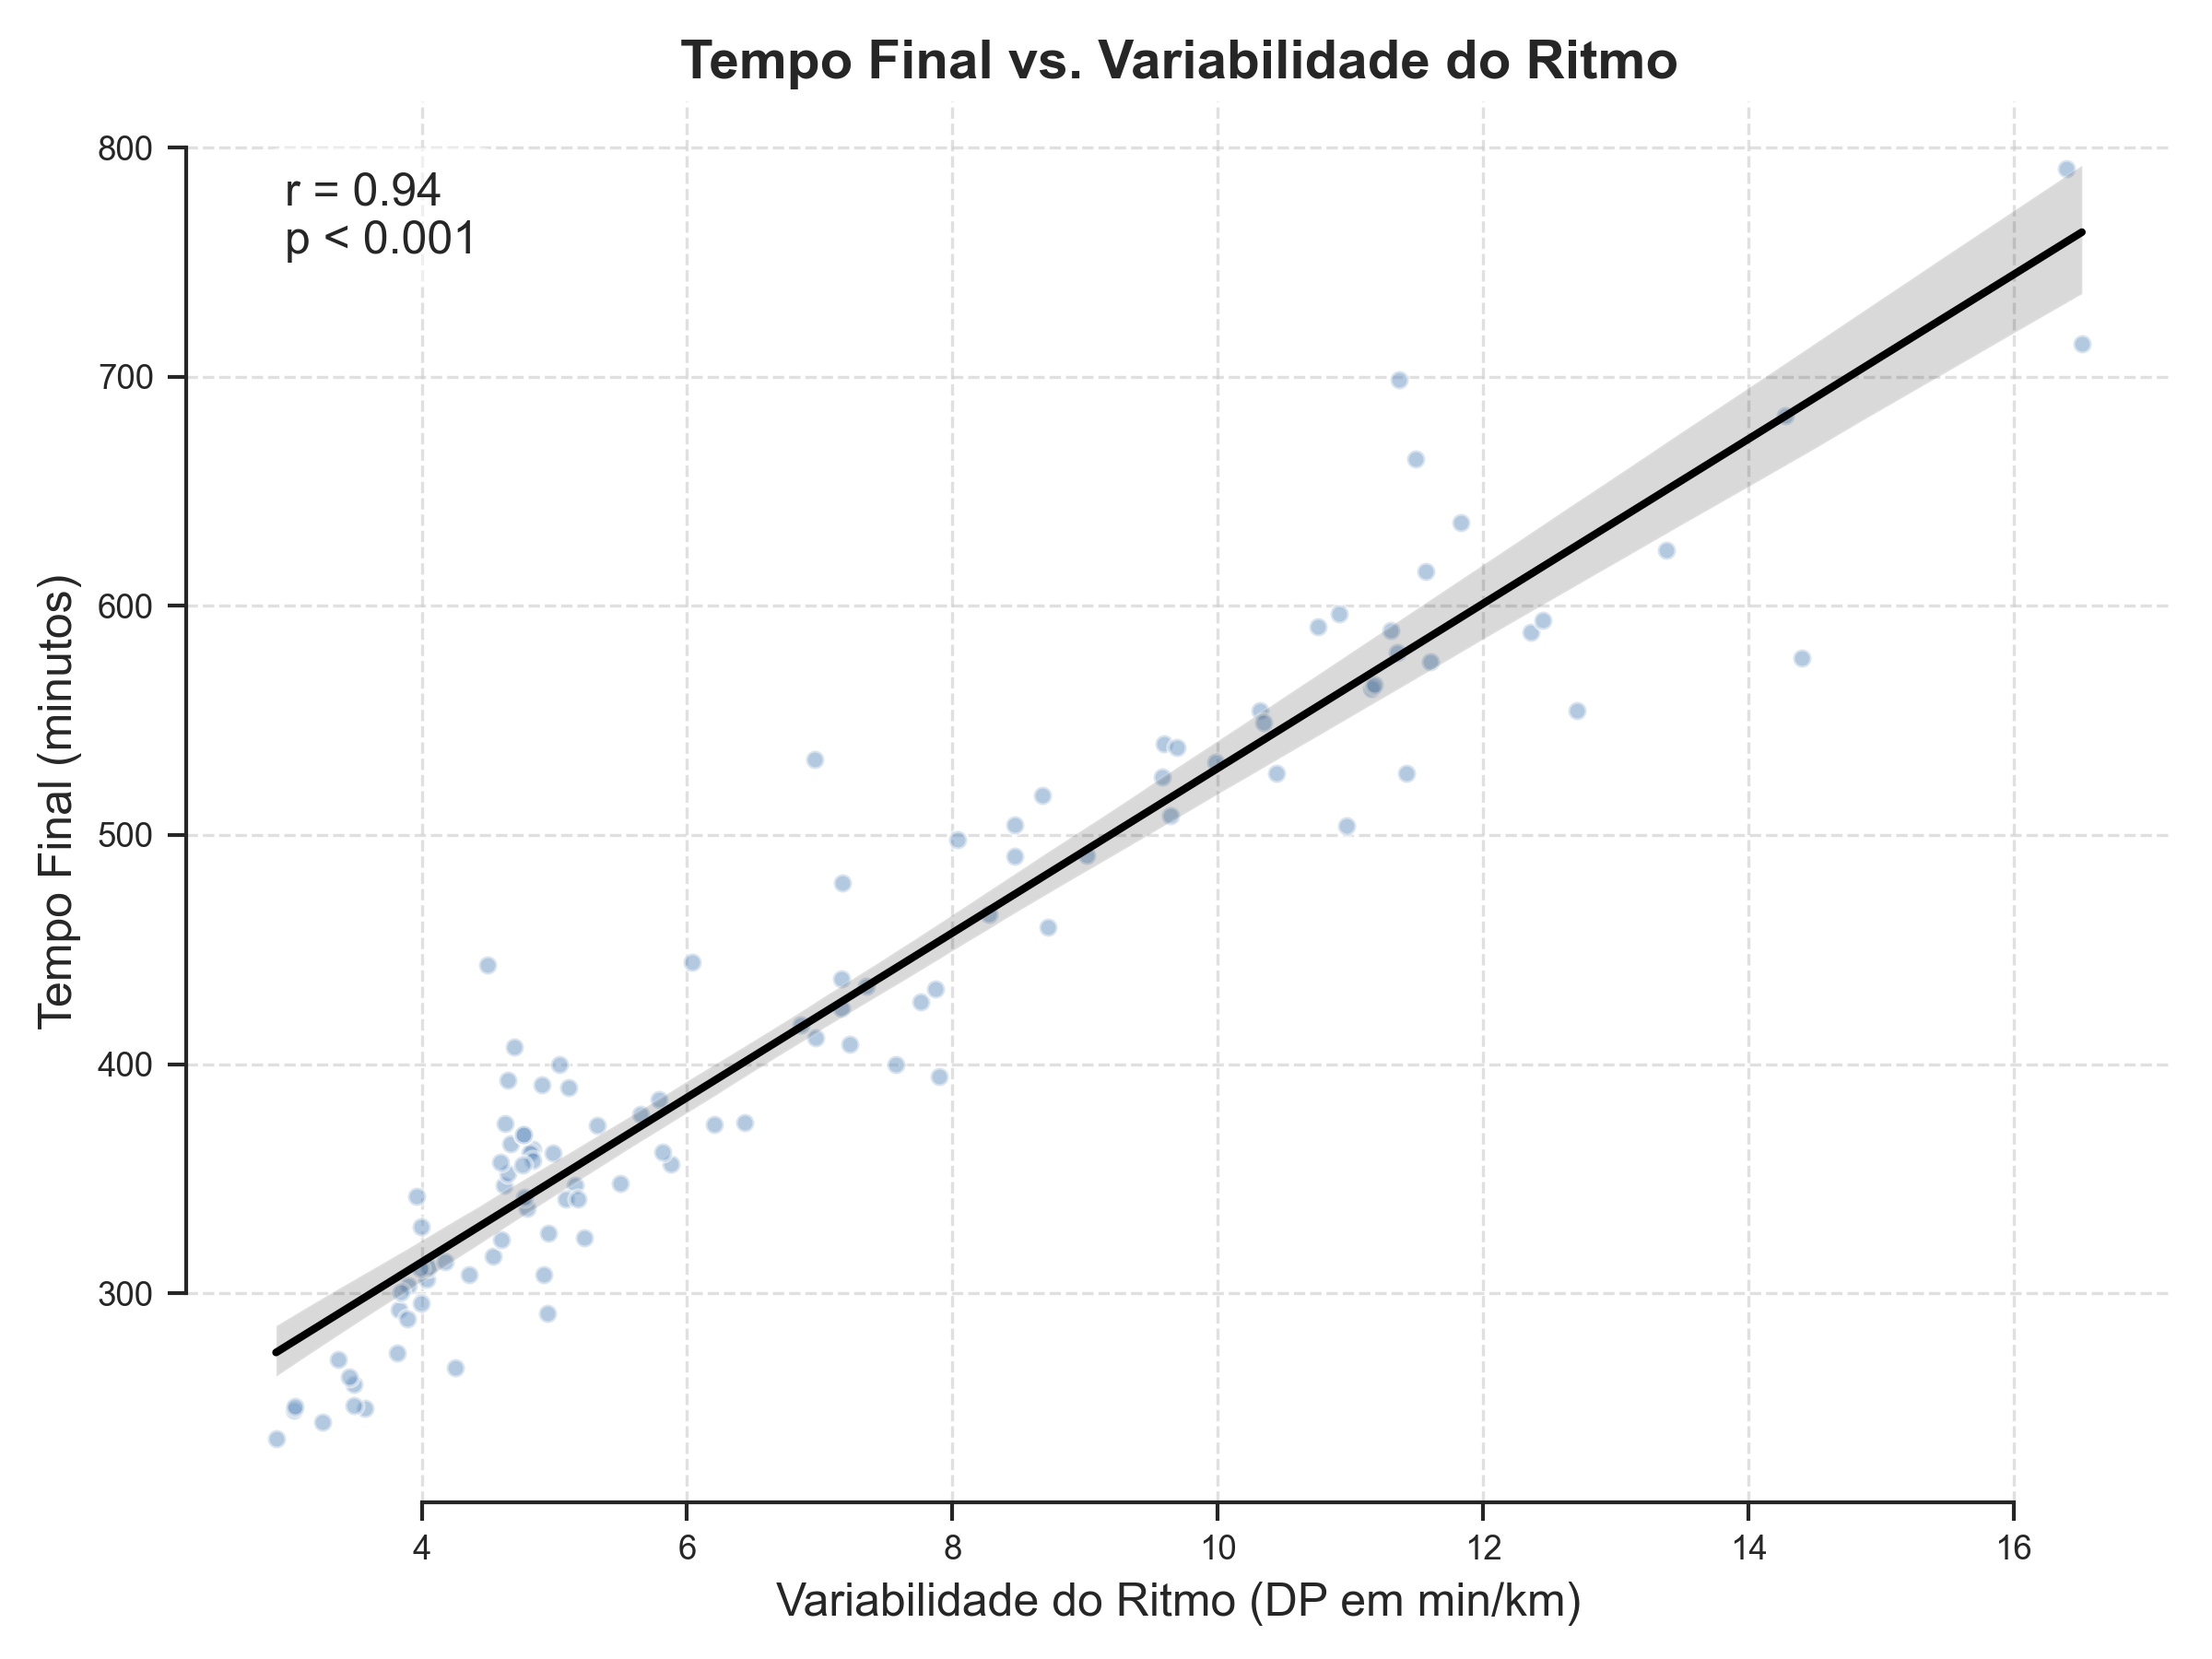
\includegraphics[width=0.8\textwidth]{Imagens/scatterplot_correlacao_ritmo.png}
    \caption{Gráfico de dispersão entre a Variabilidade do Ritmo e o Tempo Final.}
    \label{fig:scatter_variabilidade}
    \caption*{Fonte: Elaborado pelo autor (2025).}
\end{figure}

\textbf{Interpretação:} A forte correlação positiva confirma que atletas que mantiveram um ritmo mais constante ao longo da prova (menor desvio padrão) tenderam a obter tempos finais melhores (menores). A consistência do ritmo, portanto, emerge como um fator preditivo fundamental do desempenho.

\section{Análise de Agrupamento: As Personas dos Corredores}

Com o objetivo de identificar perfis de atletas com estratégias e habilidades distintas, foi realizada uma análise de clusterização K-Means. A seleção do número de clusters foi guiada pelo Método do Cotovelo, que indicou k=4 como o número ideal de agrupamentos. As variáveis utilizadas na clusterização foram selecionadas para capturar múltiplas dimensões da performance, incluindo: desempenho geral (\texttt{Tempo\_Final\_seg}), consistência (\texttt{Variabilidade\_Ritmo\_std}), gestão de prova (\texttt{diff\_relativa\_segunda\_primeira\_parte}) e especialização em terreno (\texttt{indice\_subida}, \texttt{indice\_descida}).
A análise das características médias de cada grupo (Tabela \ref{tab:perfis_clusters}) e a visualização de suas distribuições (Figura \ref{fig:boxplot_clusters}) permitiram a definição de quatro "personas" distintas de corredores.

% --- Tabela Perfis dos Clusters ---
\begin{table}[H]
\centering
\caption{Perfil médio das variáveis chave para cada cluster (k=4).}
\label{tab:perfis_clusters}
\resizebox{1.05\textwidth}{!}{%
\begin{tabular}{lccccc}
\toprule
\textbf{Variável} & \textbf{Cluster 0 (Escaladores)} & \textbf{Cluster 1 (Especialistas em Descidas)} & \textbf{Cluster 2 (Guerreiros)} & \textbf{Cluster 3 (Elite)} \\
\midrule
Tempo\_Final\_seg & 22871.56 & 30604.38 & 37286.06 & 18056.06 \\
Variabilidade\_Ritmo\_std & 325.15 & 582.33 & 711.45 & 258.11 \\
diff\_relativa... & -0.15 & -0.12 & -0.13 & -0.22 \\
indice\_subida & 0.19 & 0.28 & 0.22 & 0.20 \\
indice\_descida & -0.13 & -0.22 & -0.17 & -0.15 \\
\bottomrule
\end{tabular}
}
\caption*{Fonte: Elaborado pelo autor (2025).}
\end{table}

% --- Figura Boxplots por Cluster ---
% COMENTÁRIO: João, insira aqui o arquivo de imagem da sua grade de boxplots (In [120]).
\begin{figure}[H]
    \centering
    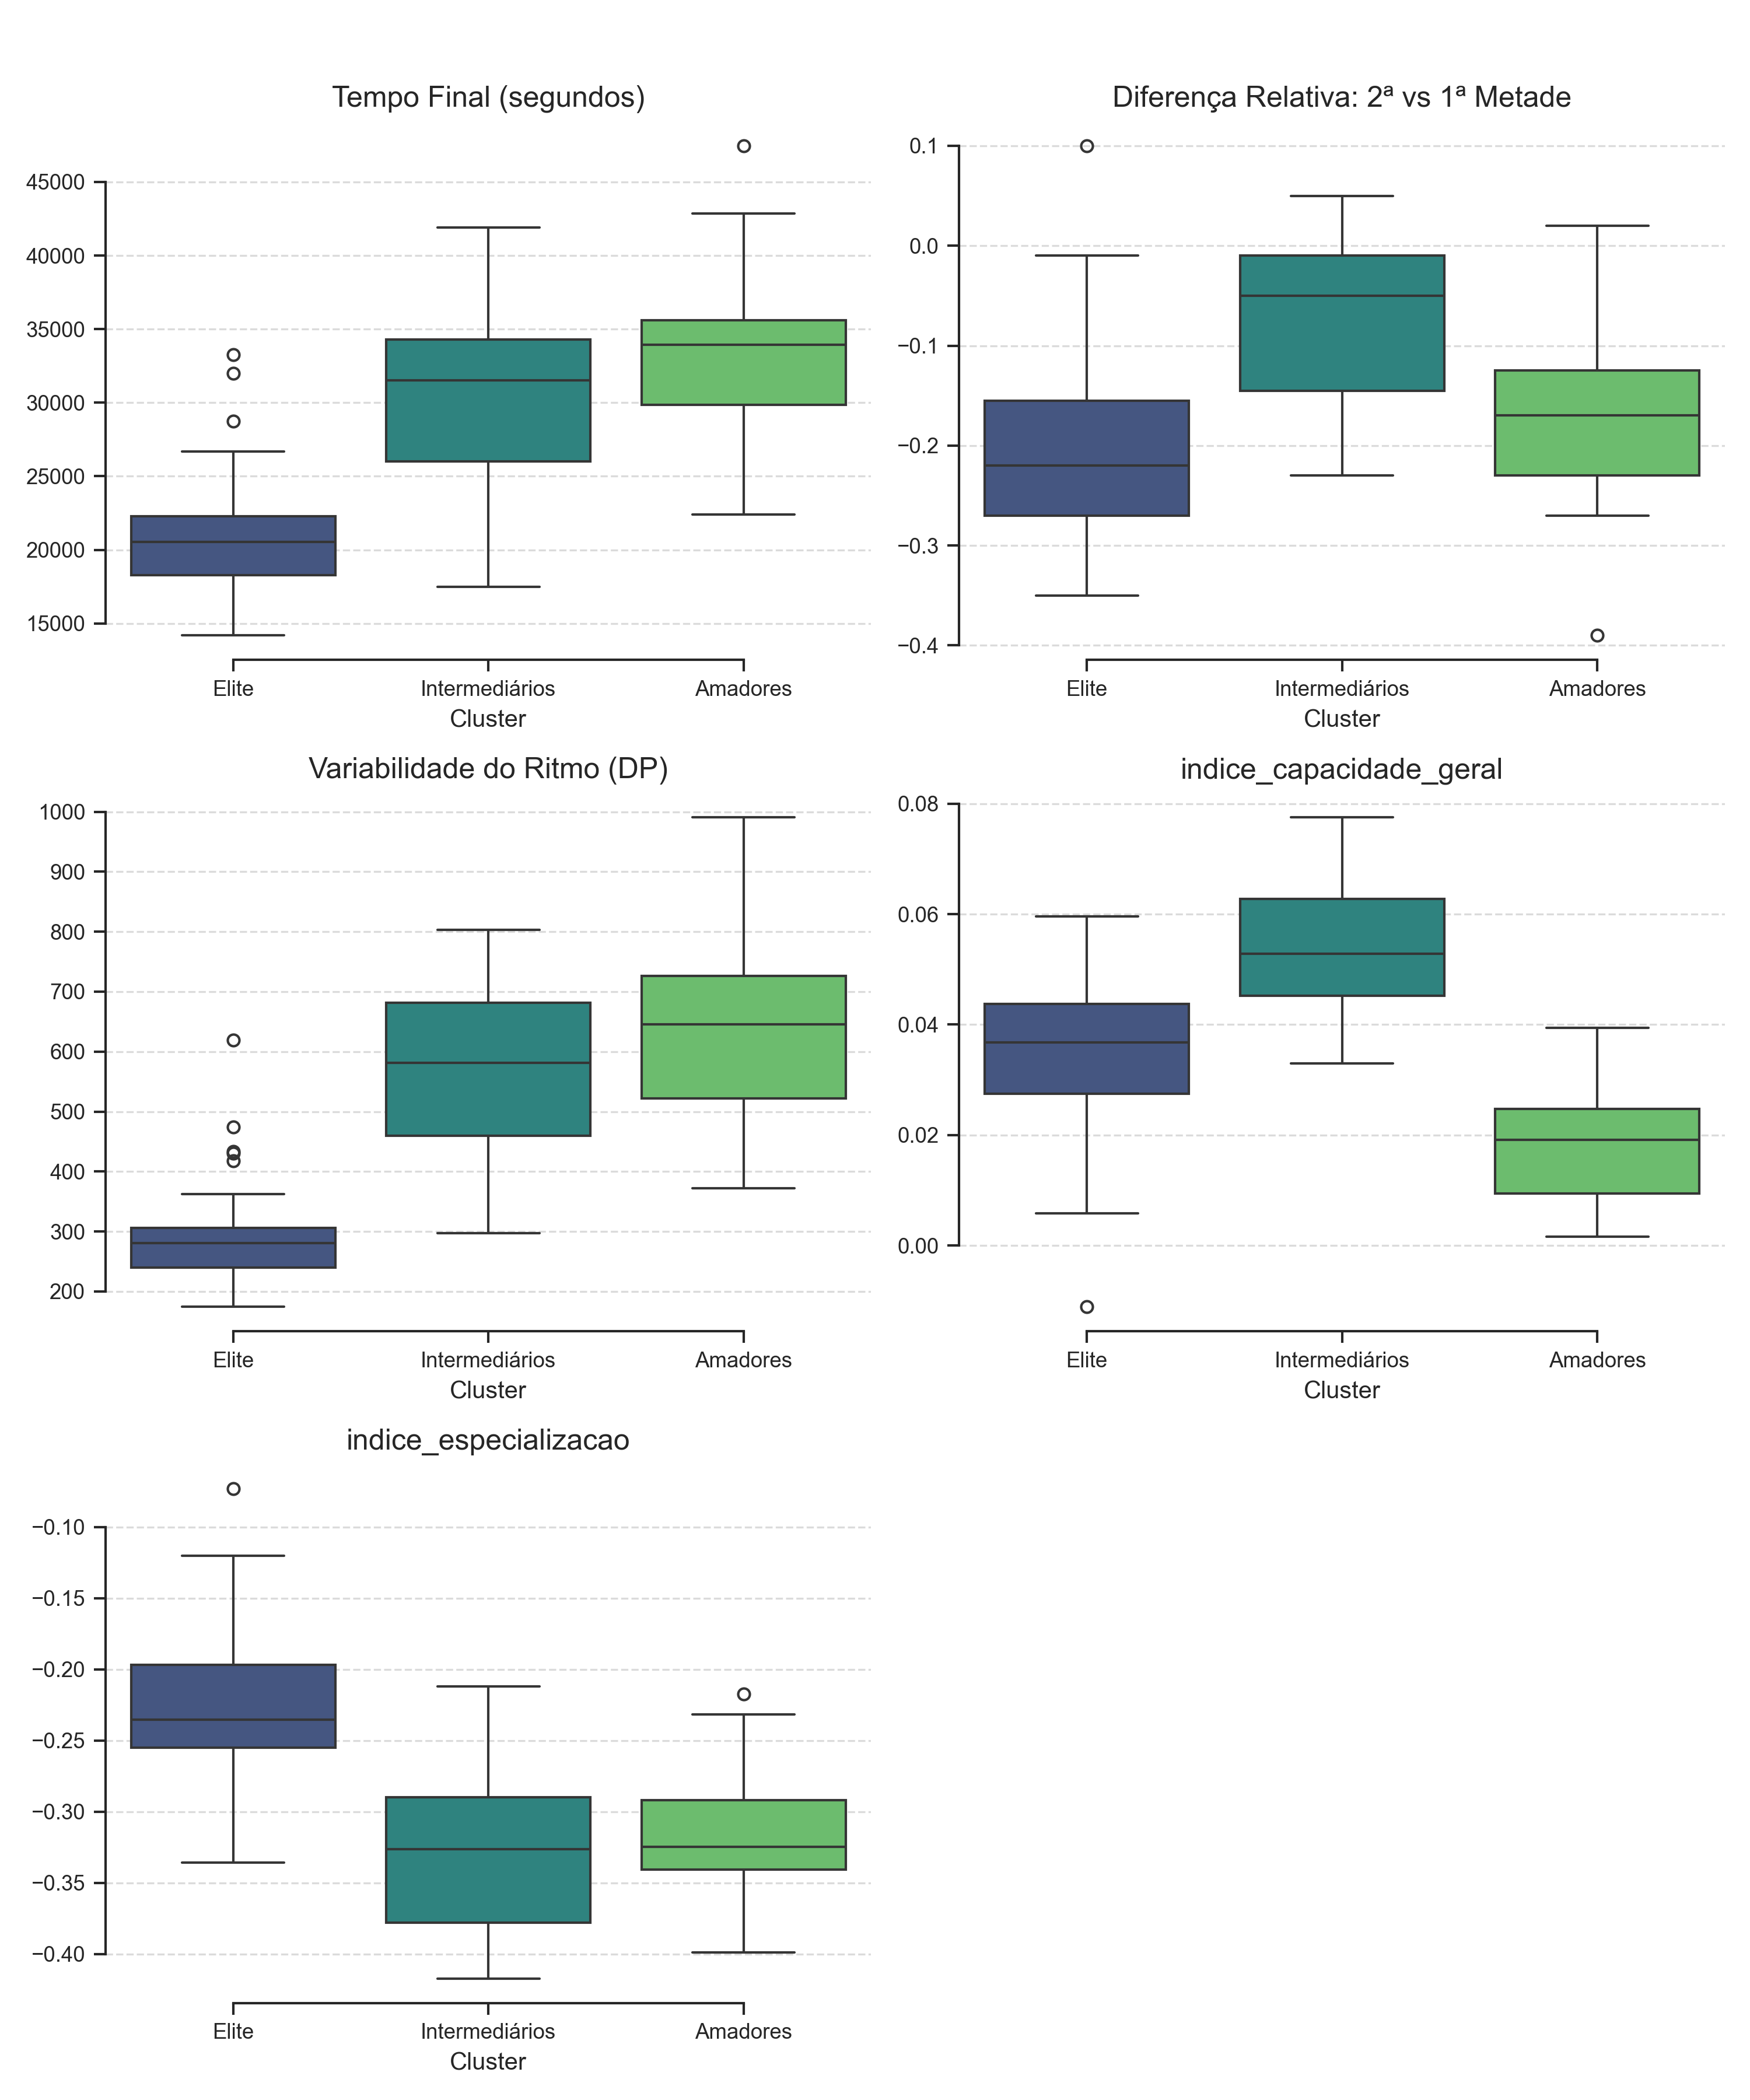
\includegraphics[width=1.05\textwidth]{Imagens/boxplot_clusters_features.png}
    \caption{Distribuição das variáveis chave por cluster.}
    \label{fig:boxplot_clusters}
    \caption*{Fonte: Elaborado pelo autor (2025).}
\end{figure}

\begin{itemize}
    \item \textbf{Cluster 3 (34 atletas): A Elite Completa.} Este grupo apresentou o menor tempo final (média de \textbf{5 horas e 56 segundos}), a menor variabilidade de ritmo e a melhor gestão de prova (\texttt{diff\_relativa} mais negativa). Seus índices de subida e descida são excelentes, demonstrando proficiência em todos os terrenos. Persona: Rápidos, estratégicos e tecnicamente completos.
    \item \textbf{Cluster 0 (34 atletas): Os Escaladores.} O segundo grupo mais rápido (média de \textbf{6 horas, 21 minutos e 11 segundos}). Sua principal característica é o excepcional desempenho em subidas, possuindo o melhor \texttt{indice\_subida} (0.19), mas um desempenho apenas mediano em descidas (\texttt{indice\_descida} de -0.13). Persona: Usam a força na subida como principal arma.
    \item \textbf{Cluster 1 (24 atletas): Os Especialistas em Descida.} Grupo intermediário (média de \textbf{8 horas, 30 minutos e 4 segundos}). Caracterizam-se por terem o pior desempenho relativo em subidas (\texttt{indice\_subida} de 0.28), mas o melhor desempenho em descidas (\texttt{indice\_descida} de -0.22). Sua alta variabilidade de ritmo é explicada por essa grande diferença de performance entre os terrenos. Persona: Atletas tecnicamente hábeis que compensam nas descidas o tempo perdido nas subidas.
    \item \textbf{Cluster 2 (17 atletas): Os Guerreiros.} O grupo com o maior tempo final (média de \textbf{10 horas, 21 minutos e 26 segundos}) e a maior variabilidade de ritmo. Seus índices de subida e descida são equilibrados, mas em um patamar de performance geral inferior. Persona: Focados em completar o desafio, com um perfil de resistência em vez de especialização técnica.
\end{itemize}

\section{Modelo Preditivo do Desempenho}

Para unificar os achados anteriores, foi ajustado um modelo de Regressão Linear Múltipla tendo o \texttt{Tempo\_Final\_seg} como variável dependente. Utilizando um processo de eliminação retrógrada (\textit{backward elimination}), buscou-se um modelo final parcimonioso e robusto, removendo-se as variáveis não significativas. O modelo final, apresentado na Tabela \ref{tab:modelo_regressao}, reteve apenas as variáveis com poder explicativo estatisticamente significativo.

% --- Tabela do Modelo Final ---
\begin{table}[H]
\centering
\caption{Sumário do Modelo Final de Regressão Linear Múltipla (OLS).}
\label{tab:modelo_regressao}
\begin{tabular}{lrrrr}
\toprule
\textbf{Variável} & \textbf{Coef.} & \textbf{Erro Padrão} & \textbf{t} & \textbf{P>|t|} \\
\midrule
\textbf{Intercepto} & 14990.00 & 620.56 & 24.15 & <0.001 \\
\texttt{Variabilidade\_Ritmo\_std} & 24.25 & 1.71 & 14.16 & <0.001 \\
\texttt{cluster\_1} & 1496.91 & 612.66 & 2.44 & 0.016 \\
\texttt{cluster\_2} & 5047.70 & 814.12 & 6.20 & <0.001 \\
\texttt{cluster\_3} & -3189.92 & 404.11 & -7.89 & <0.001 \\
\midrule
\multicolumn{5}{l}{\textbf{R² Ajustado:} 0.953} \\
\multicolumn{5}{l}{\textbf{Prob (F-statistic):} 5.55e-69} \\
\bottomrule
\end{tabular}
\caption*{Fonte: Elaborado pelo autor (2025).}
\end{table}

O modelo final apresentou um \textbf{R² ajustado de 0.953}, indicando que 95.3\% da variabilidade no tempo final dos atletas é explicada pelas variáveis do modelo. O Teste F global foi altamente significativo ($p \approx 5.55 \times 10^{-69}$), validando a significância do modelo como um todo. A interpretação dos coeficientes revela dois pilares do desempenho:
\begin{enumerate}
    \item \textbf{Consistência do Ritmo (\texttt{Variabilidade\_Ritmo\_std}):} Com um coeficiente de \textbf{24.25 (p<0.001)}, o modelo quantifica que para cada 1 segundo de aumento no desvio padrão do ritmo, o tempo final de prova aumenta, em média, em 24.25 segundos.
    \item \textbf{Perfil do Atleta (\texttt{cluster}):} As variáveis dummy dos clusters foram altamente significativas. Tomando o Cluster 0 ("Os Escaladores") como referência:
    \begin{itemize}
        \item Pertencer ao \textbf{Cluster 3 ("A Elite")} está associado a uma redução de \textbf{3.190 segundos} (aprox. 53 minutos) no tempo final (p<0.001).
        \item Pertencer ao \textbf{Cluster 1 ("Especialistas em Descida")} está associado a um aumento de \textbf{1.497 segundos} (aprox. 25 minutos) no tempo final (p=0.016).
        \item Pertencer ao \textbf{Cluster 2 ("Guerreiros")} está associado a um aumento de \textbf{5.048 segundos} (aprox. 84 minutos) no tempo final (p<0.001).
    \end{itemize}
\end{enumerate}
É notável que, após a inclusão da variável \texttt{cluster}, as variáveis demográficas como \texttt{sexo} e \texttt{faixa\_etaria} perderam significância e foram removidas do modelo final. Isso sugere que a variável \texttt{cluster} captura de forma mais eficaz e completa as diferenças de desempenho.

\section{Análise de Resíduos do Modelo Final}

A validação dos pressupostos do modelo de regressão foi realizada por meio da análise de seus resíduos.

% --- Figuras da Análise de Resíduos ---
% COMENTÁRIO: João, insira aqui os dois gráficos de análise de resíduos (In [3496]).
\begin{figure}[H]
    \centering
    \begin{minipage}{1\textwidth}
        \centering
        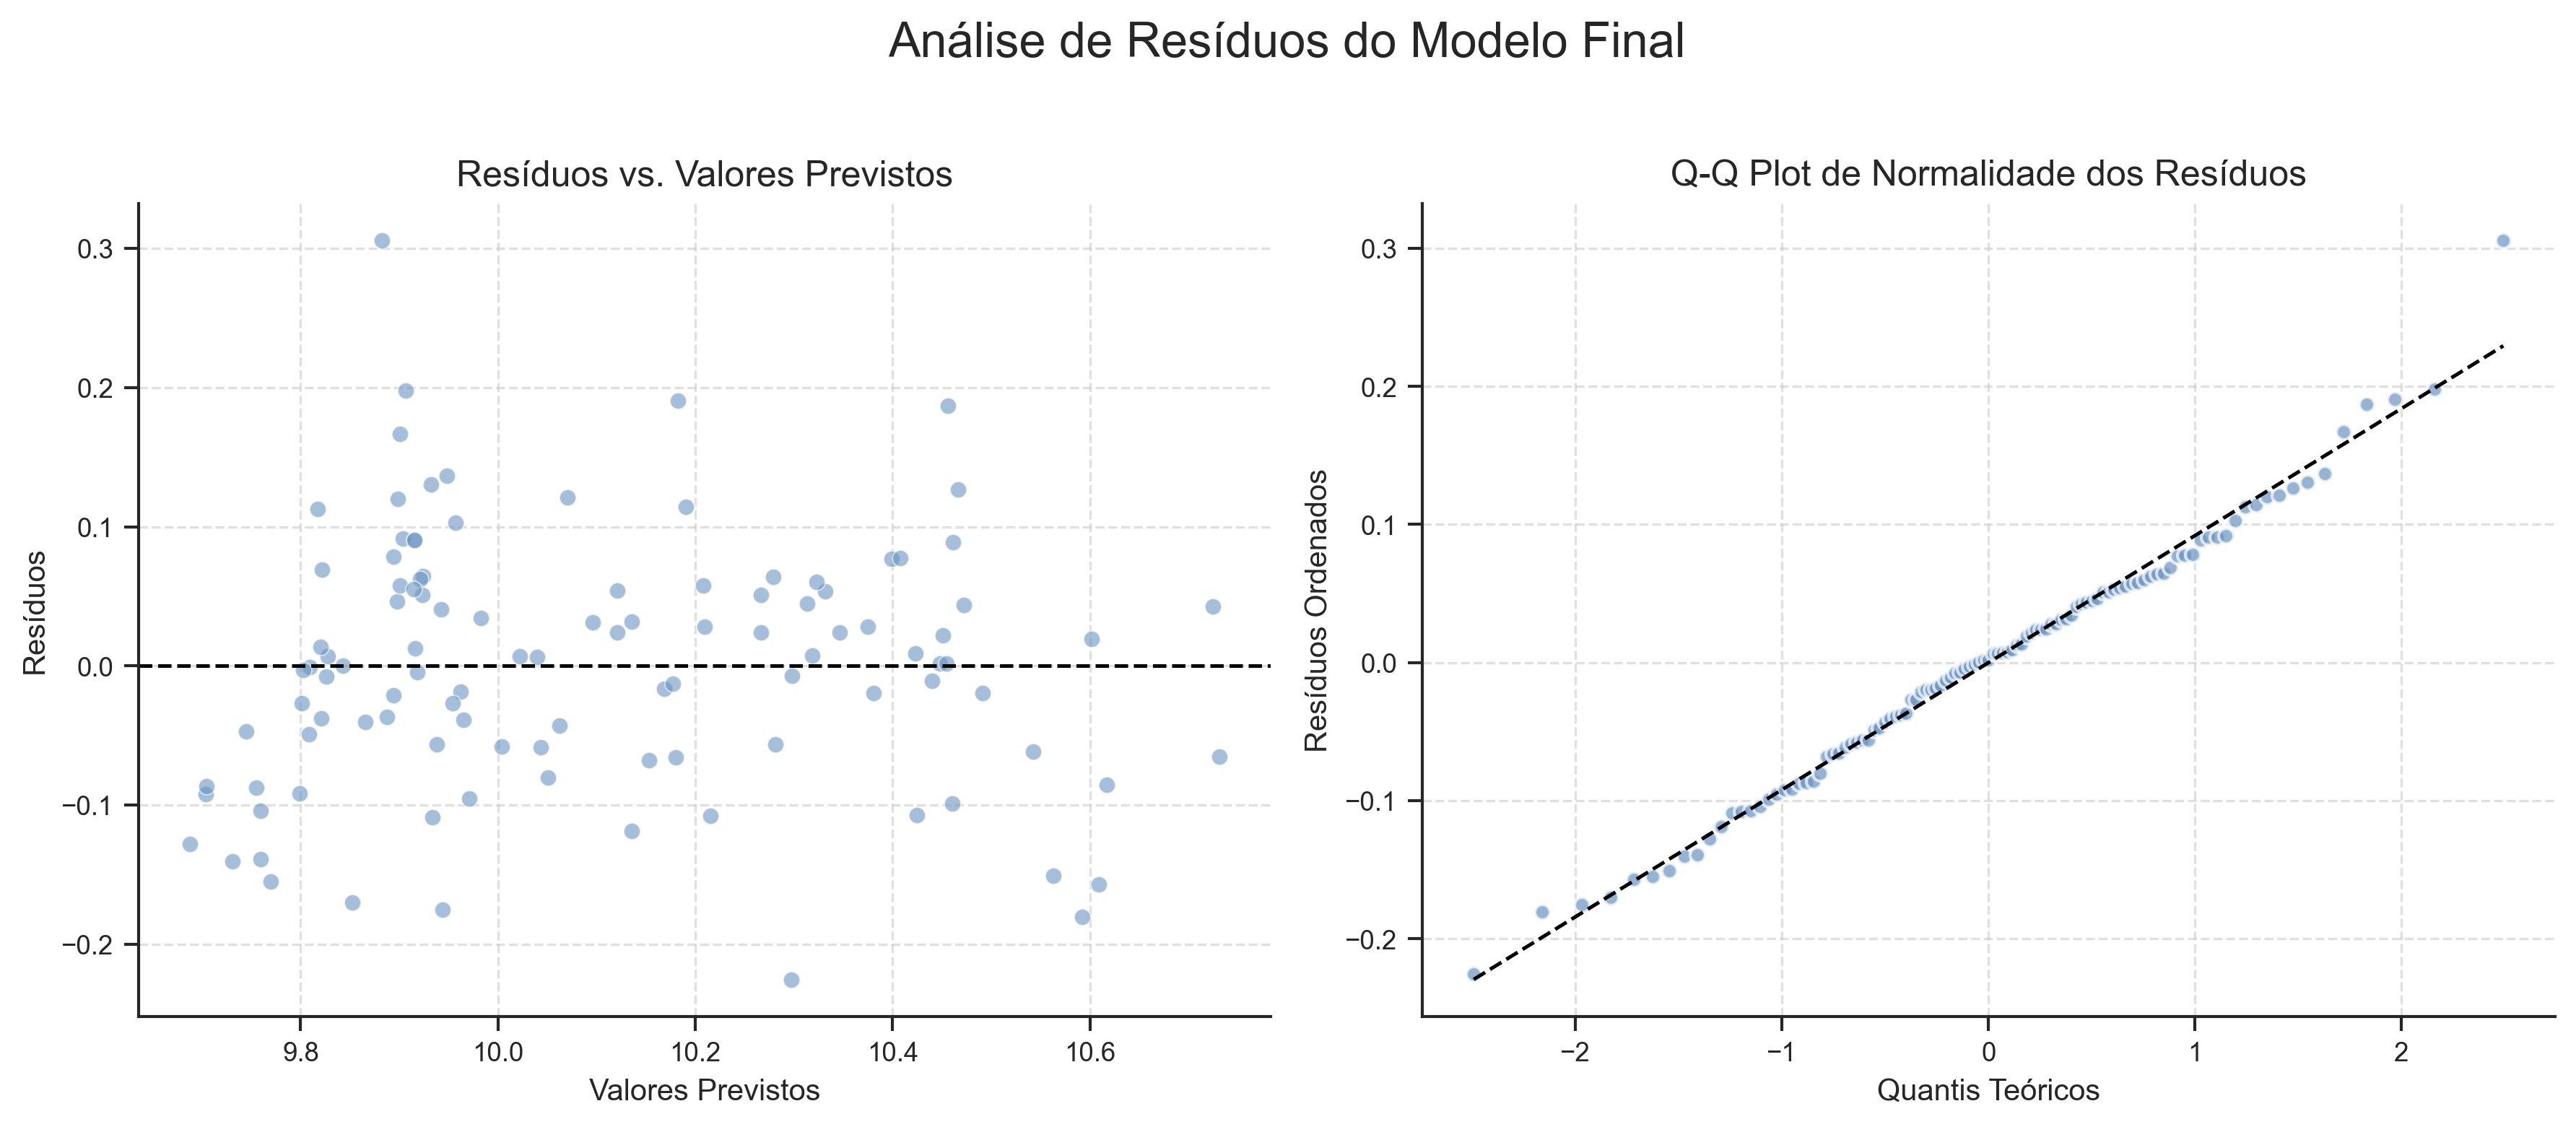
\includegraphics[width=\linewidth]{Imagens/analise_residuos_modelo.png}
        \caption{Resíduos vs. Valores Previstos.}
        \label{fig:residuos}
    \end{minipage}\hfill
    \caption*{Fonte: Elaborado pelo autor (2025).}
\end{figure}

\begin{itemize}
    \item \textbf{Linearidade e Homocedasticidade:} O gráfico de resíduos versus valores previstos (Figura \ref{fig:residuos}) exibe uma nuvem de pontos aleatoriamente dispersa em torno da linha zero, sem padrões discerníveis. Isso indica que os pressupostos de linearidade e homocedasticidade foram satisfeitos.
    \item \textbf{Independência dos Resíduos:} O valor do teste de \textbf{Durbin-Watson foi de 1.981}, muito próximo de 2, indicando ausência de autocorrelação serial nos resíduos.
    \item \textbf{Normalidade dos Resíduos:} O gráfico Q-Q (Figura \ref{fig:residuos}) mostra que, embora os pontos centrais se alinhem bem à reta teórica, há desvios nas caudas. Isso, em conjunto com os testes de Omnibus (p=0.008) e Jarque-Bera (p=0.008), confirma que o \textbf{pressuposto de normalidade dos resíduos foi violado}. Essa violação pode afetar a precisão dos intervalos de confiança e dos p-valores. Contudo, dado o altíssimo poder explicativo do modelo (R² > 0.95) e a forte significância dos preditores, as conclusões práticas sobre a importância da consistência e dos perfis de atleta permanecem robustas.
\end{itemize}
